\documentclass[journal]{IEEEtran} % ← conference を外して journal スタイル
\usepackage{amsmath, amssymb}
\usepackage{graphicx}
\usepackage{booktabs}
\usepackage[hidelinks]{hyperref}

% 図の検索パス
\graphicspath{{figs/}}

% --- TikZ 図用 ---
\usepackage{tikz}
\usetikzlibrary{arrows.meta,positioning,shapes.geometric,shapes.misc,fit}

\title{SystemDK with AITL: Physics-Aware Runtime DTCO via PID, FSM, and LLM Integration}

\author{Shinichi~Samizo% <-this % stops a space
\thanks{Independent Semiconductor Researcher. Email: \href{mailto:shin3t72@gmail.com}{shin3t72@gmail.com}.}
}

\begin{document}
\maketitle

\begin{abstract}
This paper presents SystemDK with AITL, a framework that extends conventional Design-Technology Co-Optimization (DTCO) by embedding control-theoretic loops directly into EDA flows. Compact PID controllers and FSM supervisors stabilize runtime variations (RC delay, thermal coupling, EMI/EMC disturbances). Future extensions (AITL Next) integrate LLM analyzers for adaptive PID retuning and FSM rule regeneration. The framework incorporates FEM analysis and S-parameter measurements into synthesis, P\&R, and STA, ensuring physics-aware closure. Simulations demonstrate order-of-magnitude improvements in timing stability, thermal robustness, and jitter suppression.
\end{abstract}

\begin{IEEEkeywords}
DTCO, CFET, PID control, FSM, LLM, EMI/EMC, Thermal coupling, Timing jitter, EDA.
\end{IEEEkeywords}

\section{Introduction}
Scaling to sub-2nm nodes and CFET integration introduces critical runtime effects:
\begin{itemize}
  \item RC delay variation due to interconnect scaling,
  \item Vertical thermal coupling in 3D-ICs,
  \item Stress-induced $V_{th}$ shifts,
  \item EMI/EMC noise degrading jitter and reliability.
\end{itemize}
Traditional DTCO applies static guardbands, leading to inefficiency. SystemDK with AITL embeds runtime control (PID+FSM) and, in the future, LLM-based adaptation.

\section{Proposed Framework}
\subsection{AITL Base}
PID compensates delay/thermal/voltage variations; FSM supervises modes and safety thresholds.

\subsection{AITL Next}
A lightweight LLM analyzes EDA logs, retunes PID gains $(K_p, K_i, K_d)$, and regenerates FSM rules.

\begin{figure}[t]
\centering
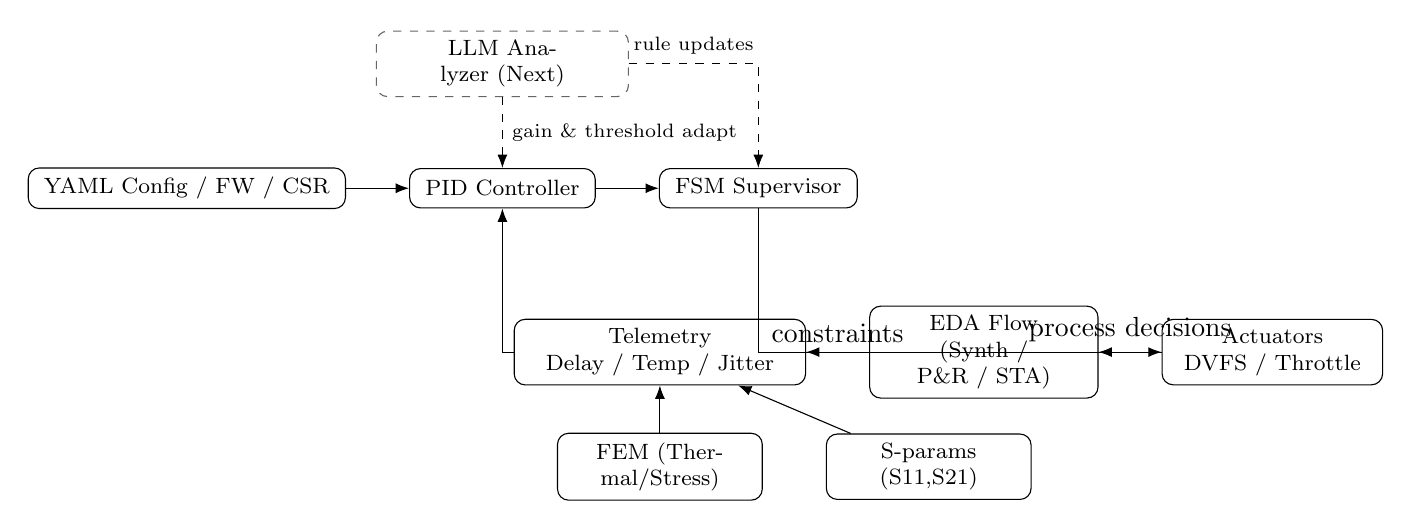
\begin{tikzpicture}[
  node distance=6mm and 8mm,
  box/.style={rounded corners, draw, minimum height=7mm, inner xsep=3mm},
  small/.style={draw, rounded corners, minimum height=5mm, inner xsep=2mm, font=\footnotesize},
  >={Latex}
]
% top control
\node[box, small] (yaml) {YAML Config / FW / CSR};
\node[box, small, right=of yaml] (pid) {PID Controller};
\node[box, small, right=of pid] (fsm) {FSM Supervisor};

% plant / EDA
\node[box, small, below=14mm of pid, xshift=20mm, text width=33mm, align=center] (tele)
{Telemetry\\ Delay / Temp / Jitter};
\node[box, small, right=of tele, text width=25mm, align=center] (eda)
{EDA Flow\\(Synth / P\&R / STA)};
\node[box, small, right=of eda, text width=24mm, align=center] (act)
{Actuators\\ DVFS / Throttle};

% physics
\node[box, small, below=of tele, text width=22mm, align=center] (fem)
{FEM (Thermal/Stress)};
\node[box, small, right=of fem, text width=22mm, align=center] (sparam)
{S-params\\(S11,S21)};

% LLM (dashed)
\node[box, small, above=9mm of pid, draw=black!60, dashed, text width=28mm, align=center] (llm)
{LLM Analyzer (Next)};

% arrows (control path)
\draw[->] (yaml) -- (pid);
\draw[->] (pid) -- (fsm);
\draw[->] (fsm) |- (act);

% telemetry loop
\draw[->] (act) -- node[midway, above, sloped]{process decisions} (eda);
\draw[->] (eda) -- node[midway, above, sloped]{constraints} (tele);
\draw[->] (tele) -| (pid);

% physics feeds
\draw[->] (fem) -- (tele);
\draw[->] (sparam) -- (tele);

% llm connections
\draw[->, dashed] (llm) -- node[right, font=\scriptsize]{gain \& threshold adapt} (pid);
\draw[->, dashed] (llm) -| node[near start, above, font=\scriptsize]{rule updates} (fsm);
\end{tikzpicture}
\caption{System overview (TikZ): control layer (PID+FSM), EDA flow, physics inputs (FEM, S-parameters), actuators, and LLM (Next).}
\label{fig:overview}
\end{figure}

\section{Analytical Models and EDA Mapping}
\subsection{RC Delay Model}
\[
t_{pd}(T,\sigma,f) = R_0 \bigl(1+\alpha_T (T-T_0)+\alpha_\sigma \sigma\bigr)\,C(f)+\Delta_{EMI}(f)
\]
Mapped to STA path-delay constraints.

\subsection{Thermal Coupling}
\[
C_{th}\frac{dT}{dt} + \frac{T-T_{amb}}{R_{th}} = P_{chip}(t)
\]
Mapped to P\&R thermal placement constraints.

\subsection{Stress-Induced $V_{th}$ Shift}
\[
\Delta V_{th}(\sigma)=\kappa \cdot \sigma
\]
Mapped to PDK/SPICE parameter updates.

\subsection{EMI Injection}
\[
v_{emi}(t)=A\sin(2\pi f_{emi} t)
\]
Mapped to SI/EMC jitter constraints.

\section{Simulation Results with EDA Implications}
\subsection{RC Delay Compensation}
\includegraphics[width=0.45\textwidth]{sim_delay_rc.png}

\subsection{Thermal Response Control}
\includegraphics[width=0.45\textwidth]{sim_thermal_response.png}

\subsection{EMI Jitter Suppression}
\includegraphics[width=0.45\textwidth]{sim_emi_jitter.png}

\subsection{FEM Analysis}
\includegraphics[width=0.45\textwidth]{fem_thermal_map.png}
\includegraphics[width=0.45\textwidth]{fem_stress_map.png}

\subsection{S-Parameter Analysis}
\includegraphics[width=0.48\textwidth]{sparam_s11s21.png}

\section{Implementation PoC}
RTL excerpt (PID controller), FSM transitions, and YAML configuration were implemented in Verilog and integrated with APB/AXI-Lite CSRs.

\section{Discussion}
\begin{itemize}
  \item Guardbands $\rightarrow$ adaptive loops,
  \item Static sign-off $\rightarrow$ dynamic runtime closure,
  \item Reliability $\rightarrow$ cross-domain resilience (delay, thermal, stress, EMI).
\end{itemize}

\section{Conclusion and Future Work}
AITL Base (PID+FSM) establishes runtime stabilization.
AITL Next will integrate lightweight LLM models for real-time EDA log analysis and control redesign.
Industrial relevance: prototype chips, EDA tool collaboration, and AI-driven DTCO.

% -------------------------
% References
% -------------------------
% まだ本文で \cite を打っていない項目も出力する
\nocite{yakimets2020cfet,irds2023,franklin2015feedback,khalil2002nonlinear,anderson2007optimal,iec61000}

\bibliographystyle{IEEEtran}
\bibliography{systemdk_aitl2025}

% -------------------------
% Biography (no photo, single author, journal style)
% -------------------------
\begin{IEEEbiographynophoto}{Shinichi Samizo}
received the M.S. degree in Electrical and Electronic Engineering from Shinshu University, Japan. He worked at Seiko Epson Corporation as an engineer in semiconductor memory and mixed-signal device development, and contributed to inkjet MEMS actuators and PrecisionCore printhead technology. He is currently an independent semiconductor researcher focusing on process/device education, memory architecture, and AI system integration. \emph{Contact:} \href{mailto:shin3t72@gmail.com}{shin3t72@gmail.com}, \href{https://github.com/Samizo-AITL}{Samizo-AITL}.
\end{IEEEbiographynophoto}

\end{document}
